\documentclass[serif, xcolor=dvipsnames]{beamer}
\makeatletter

\documentclass[xcolor={usenames,svgnames,dvipsnames}]{beamer}
\usepackage[utf8]{inputenc}
\usepackage[T1]{fontenc}
\usepackage{graphicx}
\usepackage{grffile}
\usepackage{longtable}
\usepackage{wrapfig}
\usepackage{rotating}
\usepackage[normalem]{ulem}
\usepackage{amsmath}
\usepackage{textcomp}
\usepackage{amssymb}
\usepackage{capt-of}
\usepackage{hyperref}
\usepackage{color}
\usepackage{listings}
\usepackage{mathpazo}
\usepackage{gensymb}
\usepackage{amsmath}
\usepackage{chemarr}%flechas para reacciones químicas (SFER.tex)
\bibliographystyle{plain}
\AtBeginSubsection[]{\begin{frame}[plain]\tableofcontents[currentsubsection,sectionstyle=show/shaded,subsectionstyle=show/shaded/hide]\end{frame}}
\AtBeginSection[]{\begin{frame}[plain]\tableofcontents[currentsection,hideallsubsections]\end{frame}}
\usepackage[emulate=units]{siunitx}
\sisetup{fraction=nice, decimalsymbol=comma, retain-unity-mantissa = false}
\newunit{\wattpeak}{Wp}
\newunit{\watthour}{Wh}
\newunit{\amperehour}{Ah}
\usepackage{steinmetz}
\hypersetup{colorlinks=true, linkcolor=OliveGreen, urlcolor=Blue}
\renewcommand{\thefootnote}{\fnsymbol{footnote}}
\beamertemplatenavigationsymbolsempty
\setbeamertemplate{footline}[frame number]

\setbeamercolor{alerted text}{fg=Green!50!black} \setbeamerfont{alerted text}{series=\bfseries}
\usefonttheme{serif}
\setbeamercovered{transparent}
\setbeamertemplate{navigation symbols}{}
\usefonttheme{serif} 

\setbeamercolor{palette primary}{bg=OliveGreen,fg=white}
\setbeamercolor{palette secondary}{bg=OliveGreen,fg=white}
\setbeamercolor{palette tertiary}{bg=OliveGreen,fg=white}
\setbeamercolor{palette quaternary}{bg=OliveGreen,fg=white}
\setbeamercolor{structure}{fg=OliveGreen} % itemize, enumerate, etc
\setbeamercolor{section in toc}{fg=OliveGreen} % TOC sections

\usetheme[hideothersubsections]{Goettingen}

\usepackage{tikz}

\titlegraphic{
\includegraphics[width=2.5cm]{../figs/logoEOI.jpg}}
\addtobeamertemplate{frametitle}{}{%
\begin{tikzpicture}[remember picture,overlay]
\node[anchor=south east,yshift=2pt] at (current page.south east) {
\includegraphics[width=1.5cm]{../figs/logoEOI.jpg}};
\end{tikzpicture}}


\makeatother

\usepackage[spanish]{babel}
\addto\shorthandsspanish{\spanishdeactivate{~<>}}

\begin{document}

\title[\textsc{ESF: Diseño SFB}]{\textsc{Energía Solar Fotovoltaica:}\\
\textsc{Diseño de SF de Bombeo}}


\author{\textsc{Oscar Perpiñán Lamigueiro}}
\date{}
\frame[plain]{\titlepage}

\AtBeginSection[]{
  \begin{frame}[plain]
    \frametitle{Índice}
    % \setcounter{tocdepth}{1}
    \tableofcontents[currentsection]
  \end{frame}

}


\begin{frame}
\frametitle{Potencia hidráulica}

La \textbf{potencia hidráulica}, $P_{H}$, necesaria para bombear
agua es una función de, la a\textbf{ltura vertical aparente}, $H_{v}$
y del \textbf{caudal de agua}, $Q$:\[
P_{H}=g\cdot\rho\cdot Q\cdot H_{v}\]
donde g es la aceleración de la gravedad, y $\rho$ es la densidad
del agua. 

Cambiando las unidades\[
P_{H}=2.725\cdot Q\cdot H_{V}\]


con $P_{H}$ en watios, $H_{v}$ en metros y $Q$ en $\si{\meter\cubed\per\hour}$.


\end{frame}
\begin{frame}
\frametitle{Potencia eléctrica de la motobomba}

Asumiendo que el agua bombeada sale por el conducto a una velocidad
insignificante, la potencia de salida de la bomba necesita satisfacer
$P_{H}$ más las \textbf{perdidas de fricción en la tubería}, $P_{f}$.
Consecuentemente, la \textbf{potencia eléctrica a la entrada de la
motobomba}, $P_{el}$, es:\[
P_{el}=\frac{P_{H}+P_{f}}{\eta_{mp}}\]
donde $\eta_{MP}$ es la \textbf{eficiencia de la motobomba}.

El valor de $P_{H}+P_{f}$ es la \textbf{potencia mecánica a la salida
de la bomba}. Este valor se asimila a una altura equivalente $H_{T}$
asociado a un caudal determinado:\[
H_{T}=H_{v}+H_{f}\]



\end{frame}
\begin{frame}
\frametitle{Potencia eléctrica del generador}

La \textbf{potencia eléctrica requerida por la motobomba es entregada
por un generador FV y un acondicionador de potencia}:\[
P_{el}=P_{g}^{*}\cdot\frac{G}{G^{*}}\frac{\eta_{g}}{\eta_{g}^{*}}\cdot\eta_{inv}\]


siendo $\eta_{inv}$ la \textbf{eficiencia del equipo de acondicionamiento
de potencia}.


\end{frame}
\begin{frame}
\frametitle{Caudal diario}

El \textbf{caudal diario} bombeado por este conjunto es:\[
Q_{d}=\intop_{d}\frac{P_{g}^{*}\cdot\frac{G}{G^{*}}\frac{\eta_{g}}{\eta_{g}^{*}}\cdot\eta_{inv}\cdot\eta_{mp}}{2.725\cdot H_{T}}\mathrm{dt}\]


Debido a las variaciones de la temperatura ambiente y de la irradiancia,
y también a causa del comportamiento dinámico de los pozos, \textbf{todos
los parámetros mencionados anteriormente varían a lo largo del tiempo}.
Por tanto, la resolución de la anterior ecuación es tarea dificil. 


\end{frame}
\begin{frame}
\frametitle{Altura constante}
\begin{itemize}
\item El supuesto de \textbf{altura total de bombeo constante} sólo ocurre
cuando, por un lado, las \textbf{pérdidas de fricción en la tubería
son despreciables} y, cuando por otro, el \textbf{nivel del agua dentro
del pozo se mantiene constante}. 
\item Lo primero se puede asegurar usando diámetros de tubería suficientemente
grandes: pérdidas de fricción por debajo del 5\% de la altura total
son un requisito de optimización (es decir, $H_{f}<0.05\cdot H_{T}$). 
\end{itemize}

\end{frame}
\begin{frame}
\frametitle{Altura total equivalente}

Se puede definir una \textquotedblleft{}\textbf{altura total equivalente\textquotedblright{}},
$H_{TE}$, como el hipotético valor constante que llevaría al mismo
volumen de agua bombeada:

\[
Q_{d}=\frac{P_{g}^{*}\cdot}{2.725\cdot G^{*}\cdot H_{TE}}\cdot\intop_{dia}G\cdot\frac{\eta_{g}}{\eta_{g}^{*}}\cdot\eta_{inv}\cdot\eta_{mp}\mathrm{dt}\]


Ahora, dada una $H_{TE}$, \textbf{la ecuación depende exclusivamente
de las condiciones meteorológicas y de las características de la bomba
fotovoltaica}. En la ecuación, $H_{OT}$ representa la altura desde
la salida de agua hasta el suelo.


\end{frame}
\begin{frame}
\frametitle{Caracterización de pozos}

Normalmente se realiza un \textbf{ensayo de bombeo para caracterizar
los pozos}. 

Éste consiste en extraer agua con una bomba portátil, y medir la caída
del nivel del agua en el pozo a un cierto caudal de bombeo y cuando
dicha caída se ha estabilizado. 

Tres son los parámetros que completan la caracterización del pozo
tras el ensayo: el \textbf{nivel estático}, $H_{st}$, el \textbf{nivel
dinámico}, $H_{dt}$, y el \textbf{caudal de ensayo}, $Q_{t}$.


\end{frame}
\begin{frame}
\frametitle{Caracterización de pozos}

Debe tomarse en consideración que la excesiva velocidad de extracción
de agua de un pozo puede dañar su superficie interna y provocar agujeros
que pueden llevar a un eventual colapso del pozo. Consiguientemente,
existe un \textbf{caudal máximo para cada pozo}, $Q_{max}$ . 

De hecho, la información de los ensayos mencionados de caracterización
de los pozos están, normalmente, referidos a este caudal máximo al
que se puede extraer el agua de ellos ($Q_{t}=Q_{max}$). 


\end{frame}
\begin{frame}
\frametitle{Altura total equivalente}

\textbf{Es posible calcular }$H_{TE}$ mediante:

\[
H_{TE}=H_{OT}+H_{ST}+(\frac{H_{DT}-H_{ST}}{Q_{T}})\cdot Q_{AP}+H_{f}(Q_{AP})\]


siendo $Q_{AP}$ el caudal aparente, calculado mediante $Q_{AP}=\alpha\cdot Q_{d}$,
y $\alpha=0.047\, h^{-1}$.


\end{frame}
\begin{frame}
\frametitle{Formula aproximada}

Si consideramos constantes a lo largo del tiempo las eficiencias del
generador fotovoltaico ($\dfrac{\eta_{g}}{\eta_{g}^{*}}=0.85$), motobomba
($\eta_{mp}=0.35$) y variador ($\eta_{inv}=0.9$), es posible \textbf{calcular
de forma aproximada la potencia nominal del generador} necesaria para
bombear un caudal diario $Q_{d}$ a una altura total equivalente $H_{TE}$:\[
P_{g}^{*}=\frac{10\cdot H_{TE}\cdot Q_{d}}{G_{d}/G^{*}}\]


Por ejemplo, para bombear $\SI{30}{\meter\cubed\per\Day}$ a $H_{TE}=\SI{40}{\meter}$
en un lugar de radiación diaria media $G_{d}=\SI{5}{\kilowatthour\per\meter\squared\per\Day}$
se necesita un generador fotovoltaico de: \[
P_{g}^{*}=\frac{10\cdot40\cdot30}{5}=\SI{2400}{\wattpeak}\]



\end{frame}
\begin{frame}
\frametitle{Procedimiento de diseño}
\begin{itemize}
\item A partir del caudal diario requerido y la altura total equivalente,
se calcula la potencia aproximada del generador FV.
\item Dividiendo el caudal diario requerido por la radiación diaria media,
se obtiene el caudal instantáneo medio. 
\item Con este caudal, se acude al catálogo del fabricante (por ejemplo,
la nomenclatura de Grundfos para las bombas sumergibles es SP-XX-YY,
siendo XX el caudal instantáneo nominal de la bomba) y se elige un
grupo de bombas en el entorno.
\item Con los nomogramas se elige con el modelo concreto de bomba (caudal
nominal y número de etapas) y se obtiene un valor más preciso de la
potencia del generador. Este valor debe compararse con el inicial
por comprobación de errores.
\end{itemize}

\end{frame}

\begin{frame}[plain]
\frametitle{Procedimiento de diseño}

\begin{center}
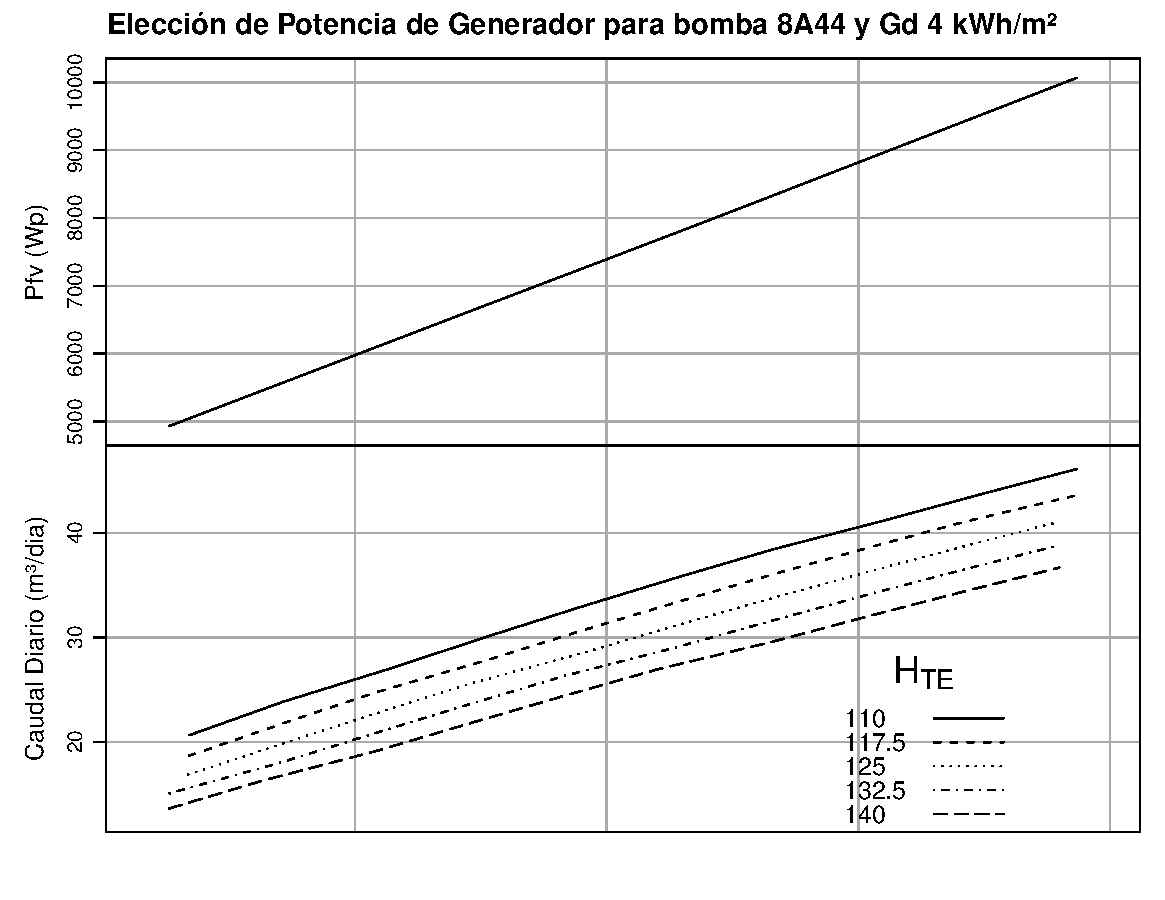
\includegraphics[scale=0.5]{../Figuras/AbacoBomba}
\par\end{center}

\end{frame}

\begin{frame}
\frametitle{Procedimiento de diseño}
\begin{itemize}
\item Como seguridad, cuando la potencia entregada por el generador es igual
al 80\% de su potencia nominal, el caudal bombeado correspondiente
no debe exceder el máximo admisible por el pozo.
\item La tensión de entrada al variador debe ser:\[
V_{DC}=\frac{\sqrt{2}V_{AC}}{1.1}\]
 luego para una bomba de tensión de $230\, V_{ac}$ se necesita una
tensión en la entrada que no sea inferior a $V_{dc}\simeq300\, V_{dc}$.
A partir de esta tensión se configura el número de módulos por serie
y el número de ramas del generador.
\item A partir del caudal $Q_{AP}$ y de la longitud de tubería necesaria,
se elige el diámetro de la misma (en curvas del fabricante) de forma
que las pérdidas sean inferiores a un porcentaje prefijado de $H_{te}$. 
\end{itemize}

\end{frame}
\begin{frame}
\frametitle{Necesidades de caudal}
\begin{itemize}
\item \textbf{OMS}: 50 litros diarios por habitante. 
\item En \textbf{crisis humanitarias}, mínimo 3 litros diarios en climas
templados y 5 litros en climas cálidos. 
\item En \textbf{programas de cooperación}, 30 a 35 litros diarios por persona. 
\item Para \textbf{sistemas fotovoltaicos}, se recomienda 25 litros diarios
por habitante (fuentes comunitarias) o 45 litros (con grifo en cada
domicilio).
\item \textbf{Contexto}: en grandes ciudades 250 litros diarios por habitante. 
\end{itemize}

\end{frame}

\end{document}
